\chapter{Analyse von Vier Gewinnt aus spieltheoretischer Sicht}


Die spieltheoretische Analyse des Spiels Vier Gewinnt erfordert eine systematische Untersuchung verschiedener strategischer Komponenten und mathematischer Aspekte. Im Folgenden Kapitel ,,Analyse von Vier Gewinnt aus spieltheoretischer Sicht'' werden die wesentlichen Elemente dieser Analyse detailliert dargestellt.
\section{Darstellung des Spiels in Normalform}



In der Normalform-Darstellung oder auch Normalform genannt, wird das Spiel als Zwei-Personen-Nullsummenspiel charakterisiert. Das bedeutet, wenn ein Spieler gewinnt ,verliert der andere automatisch . Das Spiel wird in der Normalform rein statisch beschrieben und besteht allgemein aus folgenden Elementen\autocite{gabler_normalform}:
\begin{itemize}
	\item Einer Menge Spieler $(I = {1, ..., i, ..., n})$ 
	\\ Der Wert $I$  gibt die Anzahl der Teilnehmer an.
	
	\item Für jeden Spieler i eine Menge von Strategien $(S_i)$
	\\$(S_i)$ entspricht der Strategiemenge des Spielers$i$, aus dieser er seine Züge wählen kann.
	\item Für jeden Spieler i eine Auszahlungsfunktion/ Nutzenfunktion $(u_i)$
	\\Hierbei wird jeder möglichen Strategiekombination aller Spieler einen reellen Zahlenwert zugeordnet. 
	\\  \begin{align}
		u_i &= \sum S_i \rightarrow \mathbb{R}^{n}  
\end{align}}
\end{itemize}

Ist die Normalform endlich und überschaubar, kann sie auch in einer Matrix dargestellt werden.
Die Matrix muss dabei die verschiedenen Spielsituationen und deren Ausgänge abbilden, wobei jeder Spieler in seiner Zugfolge bis zu sieben verschiedene Strategien pro Zug zur Verfügung hat. Durch die sehr große Anzahl an Strategien ist es nicht mehr überschaubar und daher eher weniger geeignet.
%*************************************************************************************************************************
\section{Komplexität des Spielbaums}
Die Komplexität des Spielbaums ist beträchtlich und wird oft als ,,mittlere Komplexität'' beschrieben. Die liegt daran, dass es eine große Anzahl an möglichen Spielzuständen gibt, aber das Spiel sich dennoch lösbar ist.\\
Die Anzahl der möglichen Konstellationen bei Vier Gewinnt beträgt laut einer Studie von John Tromp 4.531.985.219.092 (circa $4,5*10^{12}$) \autocite{thill2012reinforcement}. Aufgrund dieser enormen Zahl wird deutlich, warum eine vollständige Durchsuchung des Spielbaums für ein Vier-Gewinnt-Spiel eine Herausforderung darstellt.\\
Pro Zug gib es für den Spieler sieben Möglichkeiten. Bereits in der nach ersten Runde hat der Spielbaum $7*7 = 49$ Äste, also 49 mögliche Spielzustände. Das zeigt, dass der Spielbaum trotz der scheinbaren Einfachheit des Spiels Vier Gewinnt, recht komplex ist \autocite{thill2012reinforcement}\autocite{ruile2009viergewinnt}. Aus diesem Grund wurden Ansätze entwickelt, die den Spielbaum mithilfe von verteilten Rechensystemen effizient lösen. Ein Beispiel hierfür ist ,,Shard Solver'' \autocite{yokota2022exploration}.


\begin{figure}[H]
	\centering
	\includegraphics[width=0.9\linewidth]{"images/Baum1"}
	\caption[Spielbaum nach der 2. Tiefe]{Spielbaum nach dem 1. Zug von Spieler 1}
	\label{fig:baum1}
\end{figure}

\begin{figure}[H]
	\centering
	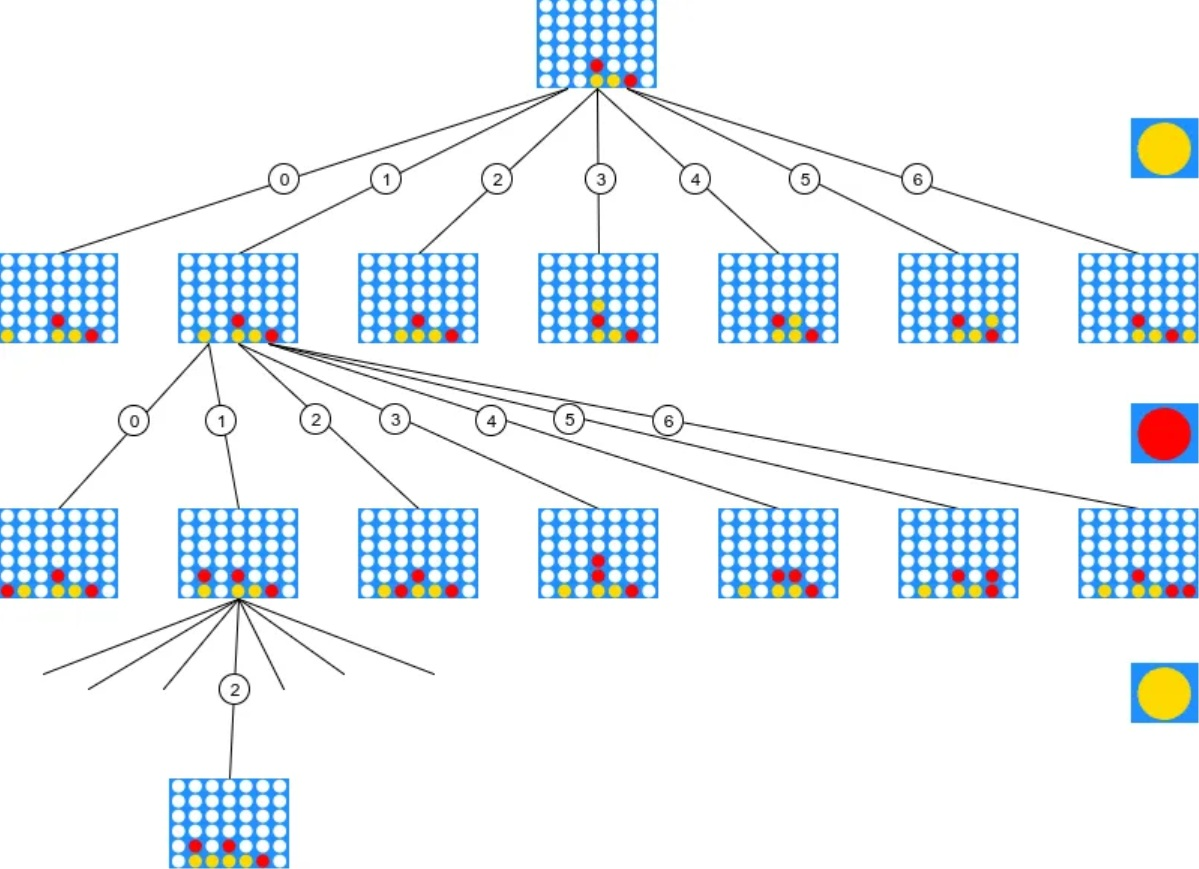
\includegraphics[width=0.9\linewidth]{"images/Baum2}
	\caption[Spielbaum nach dem 4. Zug. Quelle: \cite{vandewiele2017}]{Schematische Darstellung des Spielbaum nach dem 4. bis zum 7. Zug}
	\label{fig:Baum2}
\end{figure}



 \section{Darstellung des Spiels in Extensivform}

Die Extensivform Darstellung ist eine aufschlussreiche Methode.
Sie ermöglicht eine detaillierte Abbildung des Spielverlaufs und der Entscheidungsmöglichkeiten aller Spieler.
In dieser Form wird ein Spielbaum verwendet, der aus Knoten und Kanten besteht \autocite{einsiedler2014spieltheorie}. 
Der Baum beginnt mit einem Wurzelknoten, hier ist es ein leeres Spielfeld mit 42 freien Feldern. Die Verbindungen zwischen den Knoten, auch Kanten genannt, stellen die möglichen Züge für den Spieler dar. Die Knoten, an denen Kanten zusammenlaufen, repräsentieren eine Entscheidung eines Spielers. Die Knoten am Ende zeigen mögliche Ausgänge für das Spiel an.
Bei Vier Gewinnt stellt jede Ebene des Spielbaums einen Spielzug dar. Pro Zug gibt es immer sieben Möglichkeiten, den Spielstein zu platzieren. Das bedeutet, von jedem Knoten gehen sieben Kanten weg. Allerdings ist der Baum durch die Spielfeldgröße auf 42 mögliche Züge begrenzt.\\
Um die Extensivform praktisch nutzen zu können, werden Vereinfachungen und Optimierungen durchgeführt. Eine Möglichkeit ist es, nutzlose Züge wegzulassen. Dadurch soll der Spielbaum vereinfacht werden und sich besser für Analysen eignen \autocite{ruile2009viergewinnt}.  


\section{Strategien und Gleichgewichte}
%*******Noch Ändern************************************************************************************
Die Analyse der Strategien zeigt, dass es im Vier Gewinnt dominante Strategien gibt. Nach dem Zermelo'schen Bestimmtheitssatz lässt sich das Spiel in eine von drei Kategorien einordnen, wobei sich herausgestellt hat, dass der erste Spieler eine dominante Strategie besitzt5
. Die Nash-Gleichgewichte manifestieren sich in den optimalen Zugfolgen, wobei die Kontrolle der zentralen Spalten eine entscheidende Rolle spielt2
.


	